\capitulo{3}{Conceptos teóricos}

A continuación explicaremos algunos conceptos teóricos, es importante recalcar que los conceptos que explicamos aquí están apoyados en la explicación de los mismo que encontramos en el TFG anterior a este. \footnote{Créditos al proyecto de Roberto Arasti Blanco: eLearningQA\label{tfg-RobertoArasto}}.

\section{Definiciones básicas}
\begin{itemize}
	\item \textbf{Administración de la calidad:} es el conjunto de actividades para definir un proceso de mejora continua: aseguramiento de calidad,planificación de calidad y control de calidad.
	\item \textbf{Aseguramiento de la calidad:} establecimiento de un marco de trabajo, de procedimientos y estándares que llevan a un curso de alta calidad.
    \item \textbf{Planificación de la calidad:} selección de los procedimientos y estándares del marco de trabajo y adaptación para un curso concreto y un software específico.
    \item \textbf{Control de calidad:} procedimientos y estándares que guían al equipo de trabajo.
    \item \textbf{Medición:} el proceso por el cuál se asignan números o símbolos a los atributos las entidades del curso en línea, de tal forma que los caracteriza de manera clara a través de reglas o consultas sobre LMS.
    \item \textbf{E-learning:} proceso de enseñanza y aprendizaje impartido por medios electrónicos y digitales.
    \item \textbf{LMS:} sistema de gestión de aprendizaje que permite gestionar la enseñanza a individuos y grupos de personas, como por ejemplo Moodle, Edmodo o Blackboard.
    \item \textbf{Moodle:} es LMS creado por Martin Dougiamas en 2002 y destaca por ser el mas extendido en el mundo y por ser altamente personalizable.
    \item \textbf{API de Moodle:} conjunto de definiciones y protocolos que permite a software de terceros interactuar con el software de Moodle. Estas definiciones las encontramos en la documentación oficial\cite{moodle-api}.
    \item \textbf{MOOC:} Massive Open Online Courses o Cursos En Línea Gratuitos Masivos, hacen referencia a cursos basados en e-learning que cada vez están más extendidos en los centro educativos de todo el mundo.
    \item \textbf{Gateway:} Puerta de enlace entre datos, archivos y funcionalidades gestionadas por el servidor y los usuarios \cite{gateway}.
\end{itemize}


\section{Marco de referencia de calidad para MOOCs}
Uno de los documentos más importantes para el desarrollo de este proyecto es el Marco de referencia de calidad para MOOCs\cite{quality-reference-framework} expedido por la Alianza Europea para la calidad de los MOOCs. Para la creación de este marco se obtuvo retroalimentación de diez mil personas, todas ellas participantes de algún curso en línea, tanto como diseñador,educador,proveedor o consumidor. Con toda la información obtenida de las opiniones de las distintas personas involucradas en el proceso se concluyeron unas visiones generales para que las personas encargadas de la gestión de algún curso en línea puedan seguir.

En primer lugar hay que entender que existen 3 dimensiones a la hora de crear cursos en línea de calidad: las fases, las perspectivas y los roles.

\subsection{Fases}
En este apartado encontramos 5 fases que definen el proceso previo a la creación del curso hasta la consumición del curso por parte del alumnado.
\begin{enumerate}
    \item \textbf{Análisis:} Se comprenden tareas como la identificación y descripción de casos de uso y requerimientos, así como los límites y las necesidades. Llevado a un caso concreto podríamos pensar en la identificación de los estudiantes objetivo y su nivel académico o la planificación temporal y financiera. El estudio de la necesidad de cuestionarios y sus objetivos.
    
    \item \textbf{Diseño:} Se comprenden tareas de conceptualización y diseño de los cursos. Llevado a un caso concreto podríamos pensar en la organización de los conceptos y los roles o la definición de los objetivos de aprendizaje. El diseño de cuestionarios y actividades que animen la interacción.
    
    \item \textbf{Implementación:} Se comprenden las tareas de implementación de una versión inicial del MOOC y las pruebas del mismo. Llevado a un caso concreto podemos pensar que una vez creado el curso se implementan contenidos técnicos o recursos y se prueban. Implementación de los cuestionarios diseñados y asegurar su correcto mantenimiento.
    
    \item \textbf{Realización:} Se comprenden las tareas de puesta en funcionamiento del MOOC así como el soporte. Llevado a un caso concreto podríamos pensar en la administración del curso o la revista de niveles de competencia. Interacción del estudiantado con los cuestionarios del curso.
    
    \item \textbf{Evaluación:} En esta fase se comprenden todas las tareas de evaluación del resto de fases. Llevado a un caso concreto podríamos pensar en la evaluación del plan previo, la evaluación  de cursos o las mejoras y la optimización de un curso.
    
\end{enumerate}

\begin{figure}[H]
    \centering
    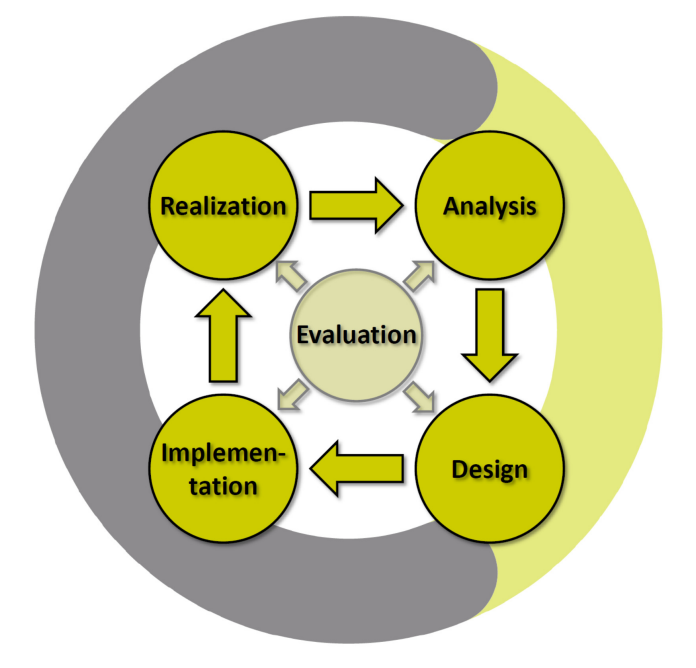
\includegraphics[width=0.75\linewidth]{fases.png}
    \caption{Fases del desarrollo del Marco de referencia de calidad para MOOCs}
    \label{fig:fases-calidad}
\end{figure}

\subsection{Perspectivas}
Las perspectivas se pueden entender como las características objetivo de cada uno de los procesos de las fases.

\begin{enumerate}
    \item \textbf{Pedagógicas}
    \item \textbf{Tecnológicas}
    \item \textbf{Estratégicas}
\end{enumerate}

Ilustremos esto con un ejemplo, en la fase de implementación, en el proceso de implementación de contenido, tenemos dos perspectivas principales: tecnológicas y pedagógicas, ya que solo se engloban aquellas tareas de implementación de los contenidos académicos y de soporte de ese contenido.

\subsection{Roles}
En esta dimensión encontramos a aquellos actores que tengan alguna responsabilidad o estén involucrados en los procesos de las fases.
\begin{enumerate}
    \item \textbf{Diseñador:} Se engloban los expertos en contenido, autores de contenido, diseñadores gráficos y expertos en plataformas LMS, así como todos los individuos que puedan contribuir al diseño del MOOC.
    \item \textbf{Facilitador:} Se engloban los expertos pedagógicos como tutores, moderadores y profesores, así como todos los individuos que puedan contribuir al proceso de aprendizaje del MOOC.
    \item \textbf{Proveedor:} Se engloban los proveedores técnicos como programadores, soporte técnico, desarrolladores de software así como todos los individuos que puedan contribuir a la toma de decisiones que lleven a la entrega del software del MOOC.
\end{enumerate}

\section{Buenas prácticas en la docencia en línea}
En la docencia en línea al igual que en el desarrollo software existen unas buenas prácticas que es conveniente seguir por el equipo educativo. Ilustraremos al lector con varias buenas prácticas basadas en la experiencia de alumnos de UBUVirtual\cite{ubu-virtual}.Además nos hemos basado en conceptos del libro Strategies for Effective Online Teaching and Learning: \cite{inbook}.
\subsection{Retroalimentaciones a tiempo}
El personal docente debe proporcionar retroalimentaciones a los estudiantes a tiempo, de esta forma se conseguirá que el alumno siga una cronología acorde a la del curso y pueda llevar una mejor organización de sus objetivos.
\subsection{Recursos actualizados}
Los recursos que el equipo docente ponga a disposición del alumnado, que pueden ser enlaces,libros,apuntes,vídeos,cuestionarios,simuladores y otros, deben estar actualizados. Para ello se deben hacer comprobaciones regularmente, de esta forma el alumnado tendrá todas las herramientas necesarias a su disposición sin incidencias. 
\subsection{Seguimiento del alumnado}
Un seguimiento continuo de la evolución del alumnado puede dar al equipo docente información clave para definir el avance del curso con el mayor éxito posible. Para realizar un buen seguimiento el docente se puede servir de cuestionarios, actividades, gráficas y otras herramientas que ofrecen los LMS.
\subsection{Priorizar la comunicación y las estrategias de interacción.}
El principal problema de la docencia en línea es la comunicación. En la docencia presencial, los alumnos ven diariamente a sus profesores y viceversa, esto facilita la comunicación y la capacidad del profesor para analizar el impacto en vivo que generan los contenidos impartidos en sus alumnos. 

Sin embargo, en la docencia en línea la información que el profesor puede obtener de las comunicaciones es más limitada, por lo que tiene que crear nuevas formas de comunicarse, que proporcionen la mayor cantidad de información posible para impartir una docencia de mayor calidad. 

Esto se tendrá que realizar mediante el uso de herramientas que todos conocemos como foros,tablones de anuncios, grupos o correos. Pero estas herramientas tan usadas no proporcionan una línea de comunicación continua y duradera en un espacio temporal como lo puede hacer conversación presencial, por lo que una muy buena práctica sería proporcionar formas de conversar entre el equipo docente y el alumnado. Esto se puede hacer implementado chats, o haciendo llamadas por medios como Skype o Teams. Además se pueden hacer reuniones semanales para discutir con lo alumnos el avance del curso y los aspectos a mejorar por ambas partes.

\subsection{Cuestionarios} 
Los cuestionarios son una herramienta muy útil para conocer una variedad de información sobre el transcurso del curso. Los cuestionarios nos ofrecen información sobre la actitud del alumnado hacia el curso, el nivel académico de los estudiantes, la evolución y otros datos. Además los LMS, como norma general, ofrecen esta funcionalidad de una forma muy completa, en el caso concreto de Moodle, existen distintas estadísticas que se pueden revisar.Ilustraremos esto con ejemplos de la documentación oficial\cite{estadisticas-examen}. Estas estadísticas proporcionan al personal académico la capacidad de detectar preguntas que están mal planteadas, entender como responden los alumnos a las preguntas y asegurar que las variantes aleatorias no afecten en exceso a los resultados:
\begin{enumerate}
    \item \textbf{Índice de facilidad:} indica el porcentaje medio de la puntuación de los estudiantes en una pregunta, lo que se puede interpretar como dificultad de la pregunta. La tabla \ref{tabla:1} muestra los intervalos de los índices de facilidad y su interpretación.
    \begin{figure}[H]
        \centering
        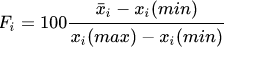
\includegraphics[width=0.7\linewidth]{img/formula-indice-facilidad.png}
        \caption{Fórmula de índice de facilidad de estadísticas de reporte de Moodle}
        \label{fig:formula-indice-facilidad}
    \end{figure}
    \item \textbf{Calificación aleatoria estimada:} muestra el resultado medio de una pregunta con respuestas aleatorias, interesante para evitar el fraude, ya que si el porcentaje es 0\% significa que los alumnos nunca podrán aprobar el cuestionario respondiendo a las preguntas aleatoriamente.
    
    \item \textbf{Índice discriminatorio:} Este índice se basa en la idea de que si un alumno ha respondido bien al resto de preguntas del cuestionario, debe responder bien a la pregunta.

    \begin{figure}[H]
        \centering
        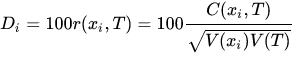
\includegraphics[width=0.70\linewidth]{img/formula-indice-discriminacion.png}
        \caption{Fórmula de índice de discriminación de estadísticas de reporte de Moodle}
        \label{fig:formula-indice-discriminacion}
    \end{figure}
    
    \item \textbf{Índice de participación:} Este índice muestra la participación que están teniendo los cuestionarios de un curso comparando los estudiantes de un curso y la participación de un cuestionario.
\end{enumerate}

\tablaSmall{Porcentaje de índices de facilidad con sus dificultades}{l c}{1}
{ \multicolumn{1}{l}{Índice de facilidad} & Interpretación\\}{ 
5\% o menos & Extremadamente difícil\\
6\% - 10\%  & Muy difícil\\
11\% - 20\% & Difícil\\
21\% - 34\%  & Moderadamente difícil\\
35\% - 65\% & Correcta para el estudiante promedio\\
66\% - 80\%  & Bastante fácil\\
81\% - 89\%  & Fácil\\
90\% - 94\%  & Muy fácil\\
95\% - 100\%  & Extremadamente fácil\\
} 

\section{Plan de calidad para cursos e-Learning}
Ya hemos visto los conceptos básicos en los que hemos basado los avances realizados en el proyecto, ahora combinaremos todos los conceptos explicados para obtener un plan de calidad claro en el que se basan las reglas implementadas de la aplicación. En este plan combinamos las distintas dimensiones del marco de referencia de calidad para MOOCs\cite{quality-reference-framework} junto con las buenas prácticas definidas. Como resultado obtenemos una tabla \ref{tabla:2} en la que encontramos los objetivo de calidad que deseamos, la responsabilidad para los roles, las perspectivas de cada uno de los objetivos y el proceso del marco de calidad para MOOCs. 

\begin{center}
    \rowcolors {2}{gray!35}{}
    \centering
    \label{tabla:2}
    \begin{longtable}{p{3cm} c c c c c}
            \caption{Objetivos de calidad en base a referencias teóricas.\\
                Leyenda:\\
                \textbf{Responsabilidad:} R=Responsable X=Involucrado\\
                \textbf{Perspectivas:} P=Pedagógica T=Tecnológica E=Estratégica
            }\\
        \hline
        Consulta & Perspectivas & Diseñador & Facilitador & Proveedor & Proceso\\
        \endhead
        \hline
        Las opciones de progreso del estudiante están activadas & P + T & R & X & & D-5 \\
        \hline
        Se proporcionan contenidos en diferentes formatos & P + T & R  & X & X & D-4\\
        \hline
        El curso tiene grupos & P & R & X & X & D-5 \\
        \hline
        El curso tiene actividades grupales & P & R & X & X & D-3 \\
        \hline
        Los estudiantes pueden ver las condiciones necesarias para completar una actividad & P & R & X & X & \\
        \hline
        Todas las actividades tienen la misma nota máxima en el calificador & P & R & X & X & \\
        \hline
        El curso tiene fechas y descripción definidas & P + E & R & X & X & \\
        \hline
        Las preguntas de los cuestionarios tienen una calificación aleatoria adecuada & P  & R & X &  & \\
        \hline        
        Las preguntas de los cuestionarios tienen retroalimentación & P & R & X & X & \\
        \hline
        Las preguntas de opción múltiple puntúan con una calificación aleatoria estimada de cero & P & R & X & X & \\
        \hline
        Los recursos están actualizados & P + T & R & X & X & I-1 \\
        \hline
        Fechas de apertura y cierre de tareas son correctas & P + T & X & R & X & R-2 \\
        \hline
        Se detallan los criterios de evaluación (rúbricas, ejemplos) & P + T & R & X & X & R-3 \\
        \hline
        El calificador no tiene demasiado anidamiento & P + E & R & X & X & \\
        \hline
        Los alumnos están divididos en grupos & T + E & X & & R & I-6 \\
        \hline
        El profesor responde en los foros dentro del límite de 48 horas lectivas desde que se plantea la duda & P + T + E & X & R & X & R-2 \\
        \hline
        Se ofrece retroalimentación de las tareas & P + T + E & X & R & X & R-2 \\
        \hline
        Las tareas están calificadas & P + T & X & R & X & R-2 \\
        \hline
        El calificador muestra cómo ponderan las diferentes tareas & P + T + E & X & R & X & R-2 \\
        \hline
        El tiempo de los cuestionarios está bien ajustado & P & R & X & X & \\
        \hline
        Los cuestionarios tienen una dificultad estimada entre unos valores umbrales & P & R & X & X & \\
        \hline
        Las preguntas de los cuestionarios son buenas discriminando & P & R & X & X & \\
        \hline
        Los índices de facilidad de las preguntas son adecuados & P + T + E & X & R & X & R-2 \\
        \hline
        Los cuestionarios tienen una participación adecuada & P + T + E & X & R & X & R-2 \\
        \hline     
        Las preguntas de los cuestionarios tienen un índice de discriminación adecuado & P + T + E & X & R & X & R-2\\
        \hline             
        La mayoría de alumnos responden a los feedbacks & P + T + E & X & X & R & E-2 \\
        \hline
        Se utilizan encuestas de opinión & P + T + E & X & X & R & E-2 \\
        \hline
    \end{longtable}
\end{center}
